\chapter{Resultados}
\label{chap:res}

Como se indica en el cap\'itulo \ref{chap:cap2}, la obtenci\'on de un grafo a partir de una imagen, es un proceso complejo. Las im\'agenes analizadas en este trabajo son aquellas en las que fue posible realizar el procedimiento de esqueletonizaci\'on, obteniendo un resultado que manten\'ia la topolog\'ia de la estructura original. Lo anterior no es un estando que pueda garantizarse para toda imagen. 


Los resultados que se presentan a continuaci\'on se separan entre tablas y figuras. Las tablas de resultados se encuentran dividas en 2 secciones dado el n\'umero de columnas. La primera secci\'on agrupa las m\'etricas y medidas indicadas en la secci\'on \ref{sec:metricasymedidas}. La segunda secci\'on muestra los porcentajes de cobertura y correctitud de los filamentos propuestos con respecto al {\it ground truth}. Es importante aclarar que aun cuando en la mayor\'ia de la tablas de resultados la columna `` \% Cobertura de Aristas'' es del 100\%, este no es siempre el caso para el algoritmo Phil, ya que no tiene como restricci\'on estricta garantizar la cobertura de cada arista del grafo, a diferencia de DeFiNe.

En cuanto a las figuras, el enfoque se dirige a presentar los resultados de DeFiNe y Phil, con \'enfasis en los filamentos correctamente encontrados por uno de los algoritmos que el otro no haya podido individualizar. Cabe aclarar que el resultado gr\'afico al ejecutar DeFiNe realiza una rotaci\'on de 90\textdegree en sentido contrarreloj adem\'as de invertir el eje vertical. Ambas modificaciones han sido corregidas con el prop\'osito de comparar los resultados entre DeFiNe, Phil y la individualizaci\'on de filamentos realizada por el experto.


En las mediciones del algoritmo {\it Phil}, se muestra el promedio de las 5 iteraciones con diferentes semillas que se realizaron. El detalle de cada iteraci\'on se encuentra en el ap\'endice \ref{chap:apendice}.
Las ejecuciones de DeFiNe y Phil fueron realizadas en un computador con un procesador {\sc Intel i5-7200U} de 4 n\'ucleos, 8GB de RAM y un disco de estado s\'lido, bajo el sistema operativo {\sc Fedora 31}.

\section{Im\'agenes Sint\'eticas}

Los resultados de la figura \ref{fig:synth-QFS-7} indicados en la tabla \ref{tab:synth-QFS-7-Results} muestran un mejor desempe\~no de DeFiNe, que encuentra un filamento m\'as que Phil con respecto a la individualizaci\'on realizada por el experto.

\begin{table}[h]
    \centering
    \begin{tabular}{|c|c|c|c|c|c|c|c|c|c|c|}
    \hline
        Algoritmo & VI & TP & FP &TN &FN & Rand	& Jaccard &	Precision &	Recall &	F1 \\ \hline
        Define 30° & 1.3859 & 5 & 6 & 55 & 12 & 0.7692  & 0.2173 & 0.4545 & 0.2941 & 0.3571\\
        Define 60° & 1.5677 & 4 & 7 & 47 & 8  & 0.7727  & 0.2105  & 0.3636  & 0.3333 & 0.3478\\ 
        Phil & 1.6360 & 10.8 & 10.4 & 104.8 & 28 & 0.7646 & 0.2484 & 0.5142 & 0.3289 & 0.3919\\
        \hline
    \end{tabular}
    \caption{Resultados de individualizaci\'on de filamentos para figura \ref{fig:synth-QFS-7}. El valor m\'aximo de VI en este caso es de 2.397895, ya que el tama\~no del {\it data set} es de 11 aristas. El n\'umero de filamentos en el {\it ground truth} es 6.}
    \label{tab:synth-QFS-7-Results}
\end{table}
\addtocounter{table}{-1}
\begin{table}[h]
    \centering
    \begin{tabular}{|c|c|c|c|c|c|c|}
    \hline
         & \multirow{4}{2cm}{\centering \% Cobertura de Aristas} & \multirow{4}{2cm}{Filamentos Propuestos} & \multirow{4}{2cm}{Filamentos Correctos} & \multirow{4}{2.5cm}{\% Correctos vs Propuestos} & \multirow{4}{2.5cm}{\centering \% Correctos vs {\it Ground Truth}} & \multirow{4}{1.2cm}{\centering Tiempo [seg]} \\
         &  &  &  & & &  \\
        Algoritmo &  &  &  & & &  \\
        &  &  &  & & &  \\ \hline
        Define 30° & 100 & 6 & 4 & 66.6667 & 66.6667 & 2.3128\\
        Define 60° & 100 & 5 & 4 & 80 & 66.6667 & 2.3380\\ 
        Phil & 100 & 6.2 & 3 & 49.1428 & 50  & 0.3569\\
        \hline
    \end{tabular}
    \caption{Resultados ({\it Continuaci\'on}) de individualizaci\'on de filamentos para figura \ref{fig:synth-QFS-7}. El n\'umero de filamentos en el {\it ground truth} es 6.}
    %\label{tab:synth-QFS-7-Results2}
\end{table}


\begin{table}[h]
    \centering
    \begin{tabular}{|c|c|c|c|c|c|c|c|c|c|c|}
    \hline
        Algoritmo & VI & TP & FP &TN &FN & Rand	& Jaccard &	Precision &	Recall &	F1 \\ \hline
        Define 30° & 1.8102 & 6 & 14 & 156  & 34 & 0.7714 & 0.1111  & 0.3 & 0.15 & 0.2\\
        Define 60° & 2.2890 & 19 & 52 & 200 & 54 & 0.6738 & 0.152 & 0.2676  & 0.2602  & 0.2638\\ 
        Phil & 2.2164 & 22.8 & 40 & 240.4 & 61.4 & 0.7227 & 0.1838 & 0.3607 & 0.2724 & 0.3100\\
        \hline
    \end{tabular}
    \caption{Resultados de individualizaci\'on de filamentos para figura \ref{fig:synth-Define-1b}.El valor m\'aximo de VI en este caso es de 3.044522, ya que el tama\~no del {\it data set} es de 17 aristas. El n\'umero de filamentos en el {\it ground truth} es 5.}
    \label{tab:synth-Define-1b}
\end{table}
\addtocounter{table}{-1}
\begin{table}[h]
    \centering
    \begin{tabular}{|c|c|c|c|c|c|c|}
    \hline
         & \multirow{4}{2cm}{\centering \% Cobertura de Aristas} & \multirow{4}{2cm}{Filamentos Propuestos} & \multirow{4}{2cm}{Filamentos Correctos} & \multirow{4}{2.5cm}{\% Correctos vs Propuestos} & \multirow{4}{2.5cm}{\centering \% Correctos vs {\it Ground Truth}} & \multirow{4}{1.2cm}{\centering Tiempo [seg]} \\
         &  &  &  & & &  \\
        Algoritmo &  &  &  & & &  \\
        &  &  &  & & &  \\ \hline
        Define 30° & 100 & 11 & 2 & 18.1818 & 40 & 2.8275\\
        Define 60° & 100 & 7 & 2 & 28.5714 & 40 & 3.6597\\ 
        Phil & 100 & 9.2 & 3 & 32.6667 & 60 & 0.5071\\
        \hline
    \end{tabular}
    \caption{Resultados ({\it Continuaci\'on}) de individualizaci\'on de filamentos para figura \ref{fig:synth-Define-1b}. El n\'umero de filamentos en el {\it ground truth} es 5.}
    %\label{tab:synth-QFS-7-Results2}
\end{table}

\section{Im\'agenes Reales}

%recordar que define es base de BFS-Overlap-pairwise-total-
% recordarr que son 5 iteraciones y se estan promediando los resultados, conectar con la columna cobertura 



\subsection{Microt\'ubulos}

%Valor m\'ax de VI para \ref{tab:SpinningMarchantiaResults1} es 3.4965.
%N\'umero de filamentos en el {\it Ground Truth} de la figura SpinningMarchanria es 12.
%Define y Phil presentan una propuesta de filamento para el ....

\begin{table}[h]
    \centering
    \begin{tabular}{|c|c|c|c|c|c|c|c|c|c|c|}
    \hline
        Algoritmo & VI & TP & FP &TN &FN & Rand	& Jaccard &	Precision &	Recall &	F1 \\ \hline
        Define 30° & 2.2870  & 15 & 38 & 523 & 54 & 0.8539 & 0.1401 & 0.2830 & 0.2173 & 0.2459\\
        Define 60° & 0.9696 & 23 & 12 & 465 & 28 & 0.9242 & 0.3650 & 0.6571 & 0.4509  & 0.5348 \\ 
        Phil & 1.8376 & 43 & 54 & 815 & 78 & 0.8666 & 0.2457 & 0.4432 & 0.3553 & 0.3944 \\
        \hline
    \end{tabular}
    \caption{Resultados de individualizaci\'on de filamentos para figura \ref{fig:SpinningMarchantia}. El valor m\'aximo de VI en este caso es de 3.4965, ya que el tama\~no del {\it data set} es de 29 aristas. El n\'umero de filamentos en el {\it ground truth} es 12.}
    \label{tab:SpinningMarchantiaResults1}
\end{table}
\addtocounter{table}{-1}
\begin{table}[h]
    \centering
    \begin{tabular}{|c|c|c|c|c|c|c|}
    \hline
         & \multirow{4}{2cm}{\centering \% Cobertura de Aristas} & \multirow{4}{2cm}{Filamentos Propuestos} & \multirow{4}{2cm}{Filamentos Correctos} & \multirow{4}{2.5cm}{\% Correctos vs Propuestos} & \multirow{4}{2.5cm}{\centering \% Correctos vs {\it Ground Truth}} & \multirow{4}{1.2cm}{\centering Tiempo [seg]} \\
         &  &  &  & & &  \\
        Algoritmo &  &  &  & & &  \\
        &  &  &  & & &  \\ \hline
        Define 30° & 100 & 16 & 9 & 56.25       & 75          & 4.1087 \\
        Define 60° & 100 & 12 & 5 & 41.6666 & 41.6666 & 5.9999 \\ 
        Phil & 100 & 12 & 7 & 58.3333 & 58.3333 & 0.6558 \\
        \hline
    \end{tabular}
    \caption{Resultados ({\it Continuaci\'on}) de individualizaci\'on de filamentos para figura \ref{fig:SpinningMarchantia}. El n\'umero de filamentos en el {\it ground truth} es 12.}
    %\label{tab:SpinningMarchantiaResults2}
\end{table}



%Valor m\'ax de VI para \ref{tab:field3t0filtered1} es 3.7612.
%N\'umero de filamentos en el {\it Ground Truth} de la figura field3t0 es 12.


\begin{table}[h]
    \centering
    \begin{tabular}{|c|c|c|c|c|c|c|c|c|c|c|}
    \hline
        Algoritmo & VI & TP & FP &TN &FN & Rand	& Jaccard &	Precision &	Recall &	F1 \\ \hline
        Define 30° & 2.0180 & 16 & 19 & 917 & 83 & 0.9014 & 0.9014 & 0.4571 & 0.1616 & 0.2388\\
        Define 60° &  2.8959 & 57 & 89 & 1359 & 148 & 0.8566 & 0.1938 & 0.3904 & 0.2780 & 0.3247\\ 
        Phil & 2.2788 & 96 & 89.4 & 1894.6 & 199 & 0.8738 & 0.2535 & 0.5130 & 0.3346 & 0.4037 \\
        \hline
    \end{tabular}
    \caption{Resultados de individualizaci\'on de filamentos para figura \ref{fig:field3t0filtered1}. El valor m\'aximo de VI en este caso es de 3.7612, ya que el tama\~no del {\it data set} es de 40 aristas. El n\'umero de filamentos en el {\it ground truth} es 12.}
    \label{tab:field3t0filtered1}
\end{table}
\addtocounter{table}{-1}
\begin{table}[h]
    \centering
    \begin{tabular}{|c|c|c|c|c|c|c|}
    \hline
         & \multirow{4}{2cm}{\centering \% Cobertura de Aristas} & \multirow{4}{2cm}{Filamentos Propuestos} & \multirow{4}{2cm}{Filamentos Correctos} & \multirow{4}{2.5cm}{\% Correctos vs Propuestos} & \multirow{4}{2.5cm}{\centering \% Correctos vs {\it Ground Truth}} & \multirow{4}{1.2cm}{\centering Tiempo [seg]} \\
         &  &  &  & & &  \\
        Algoritmo &  &  &  & & &  \\
        &  &  &  & & &  \\ \hline
        Define 30° &  1 & 23 & 6 & 26.0869 & 50 & 5.0306 \\
        Define 60° &  1 & 16 & 6 & 37.5 & 50 & 16.2042\\ 
        Phil &  1 & 15 & 7.8 & 52.0952 & 65 & 0.9693 \\
        \hline
    \end{tabular}
    \caption{Resultados ({\it Continuaci\'on}) de individualizaci\'on de filamentos para figura \ref{fig:field3t0filtered1}. El n\'umero de filamentos en el {\it ground truth} es 12.}
    %\label{tab:field3t0filtered1-2}
\end{table}


%Valor m\'ax de VI para \ref{tab:field3t0filtered2} es 1.9459.
%N\'umero de filamentos en el {\it Ground Truth} de la figura field3t0 es 5.

La individualizaci\'on de filamentos para la figura \ref{fig:field3t0filtered2} resulta en un empate entre Phil y la configuraci\'on de DeFiNe con 60\textdegree, encontrando 4 de 5 filamentos cada uno, mientras que DeFiNe con 30\textdegree como umbral encuentra s\'olo 3 de 5 filamentos. El filamento faltante en Phil y DeFiNe-60\textdegree es el que esta compuesto s\'olo por la arista 0, y en ambos casos el filamento propuesto es con las aristas 0-3.


En el caso de DeFiNe con 30\textdegree, se pierde un filamento correcto al asignar la arista 0 con la arista 3, dado que es una combinaci\'on m\'as recta que la que forman las aristas 3 y 1, que son las que constituyen el filamento correcto.

\begin{figure*}[h!]
    \centering
    \begin{subfigure}[t]{0.3\textwidth}
        \centering
        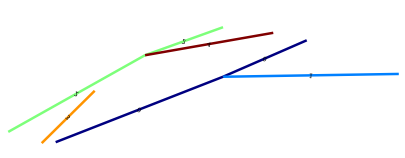
\includegraphics[scale=0.5]{resultImages/field3-t0-2cellBcrop-filtered-2-DeFiNe30.png}
        \caption{Individualizaci\'on mediante DeFiNe con 30\textdegree}
        \label{fig:field3t0filtered2Results-a}
    \end{subfigure}%
    ~ 
    \begin{subfigure}[t]{0.3\textwidth}
        \centering
        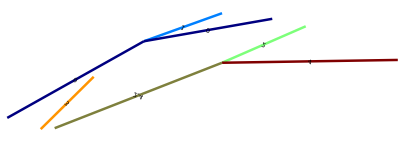
\includegraphics[scale=0.5]{resultImages/field3-t0-2cellBcrop-filtered-2-DeFiNe60.png}
        \caption{Individualizaci\'on mediante DeFiNe con 60\textdegree}
        \label{fig:field3t0filtered2Results-b}
    \end{subfigure}
    ~ 
    \begin{subfigure}[t]{0.3\textwidth}
        \centering
        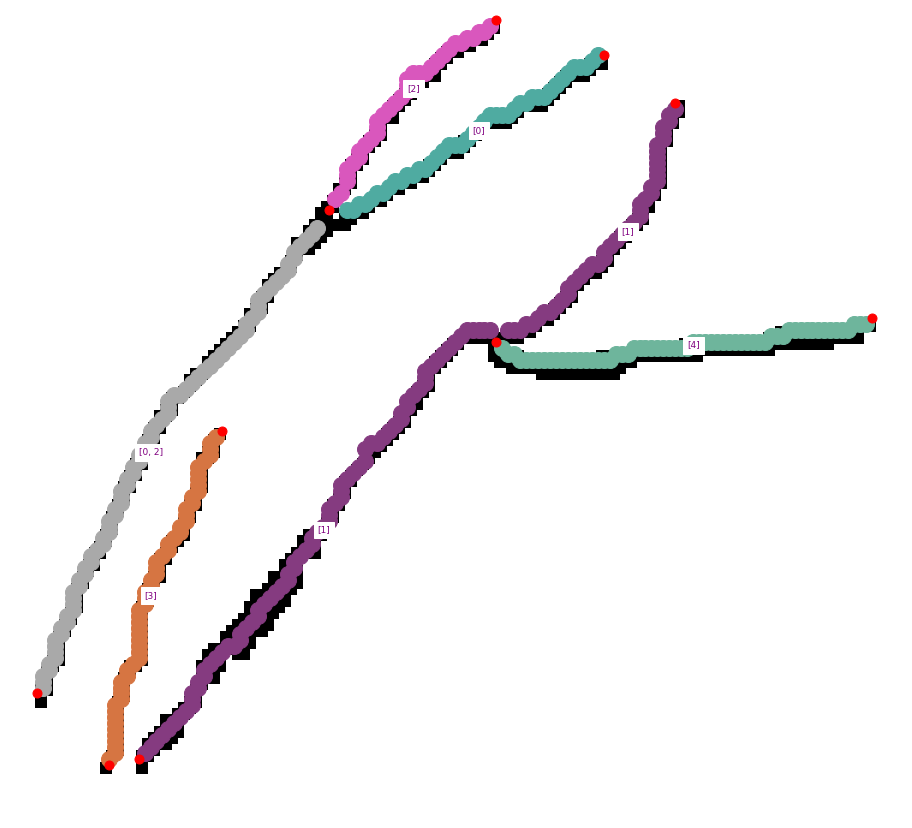
\includegraphics[height=1.5in]{resultImages/field3-t0-2cellBcrop-filtered-2-phil-s1271-v05-antLabeled.png}
        \caption{Individualizaci\'on con Phil}
        \label{fig:field3t0filtered2Results-c}
    \end{subfigure}
    \vskip\baselineskip
    
    \begin{subfigure}[t]{0.3\textwidth}
        \centering
        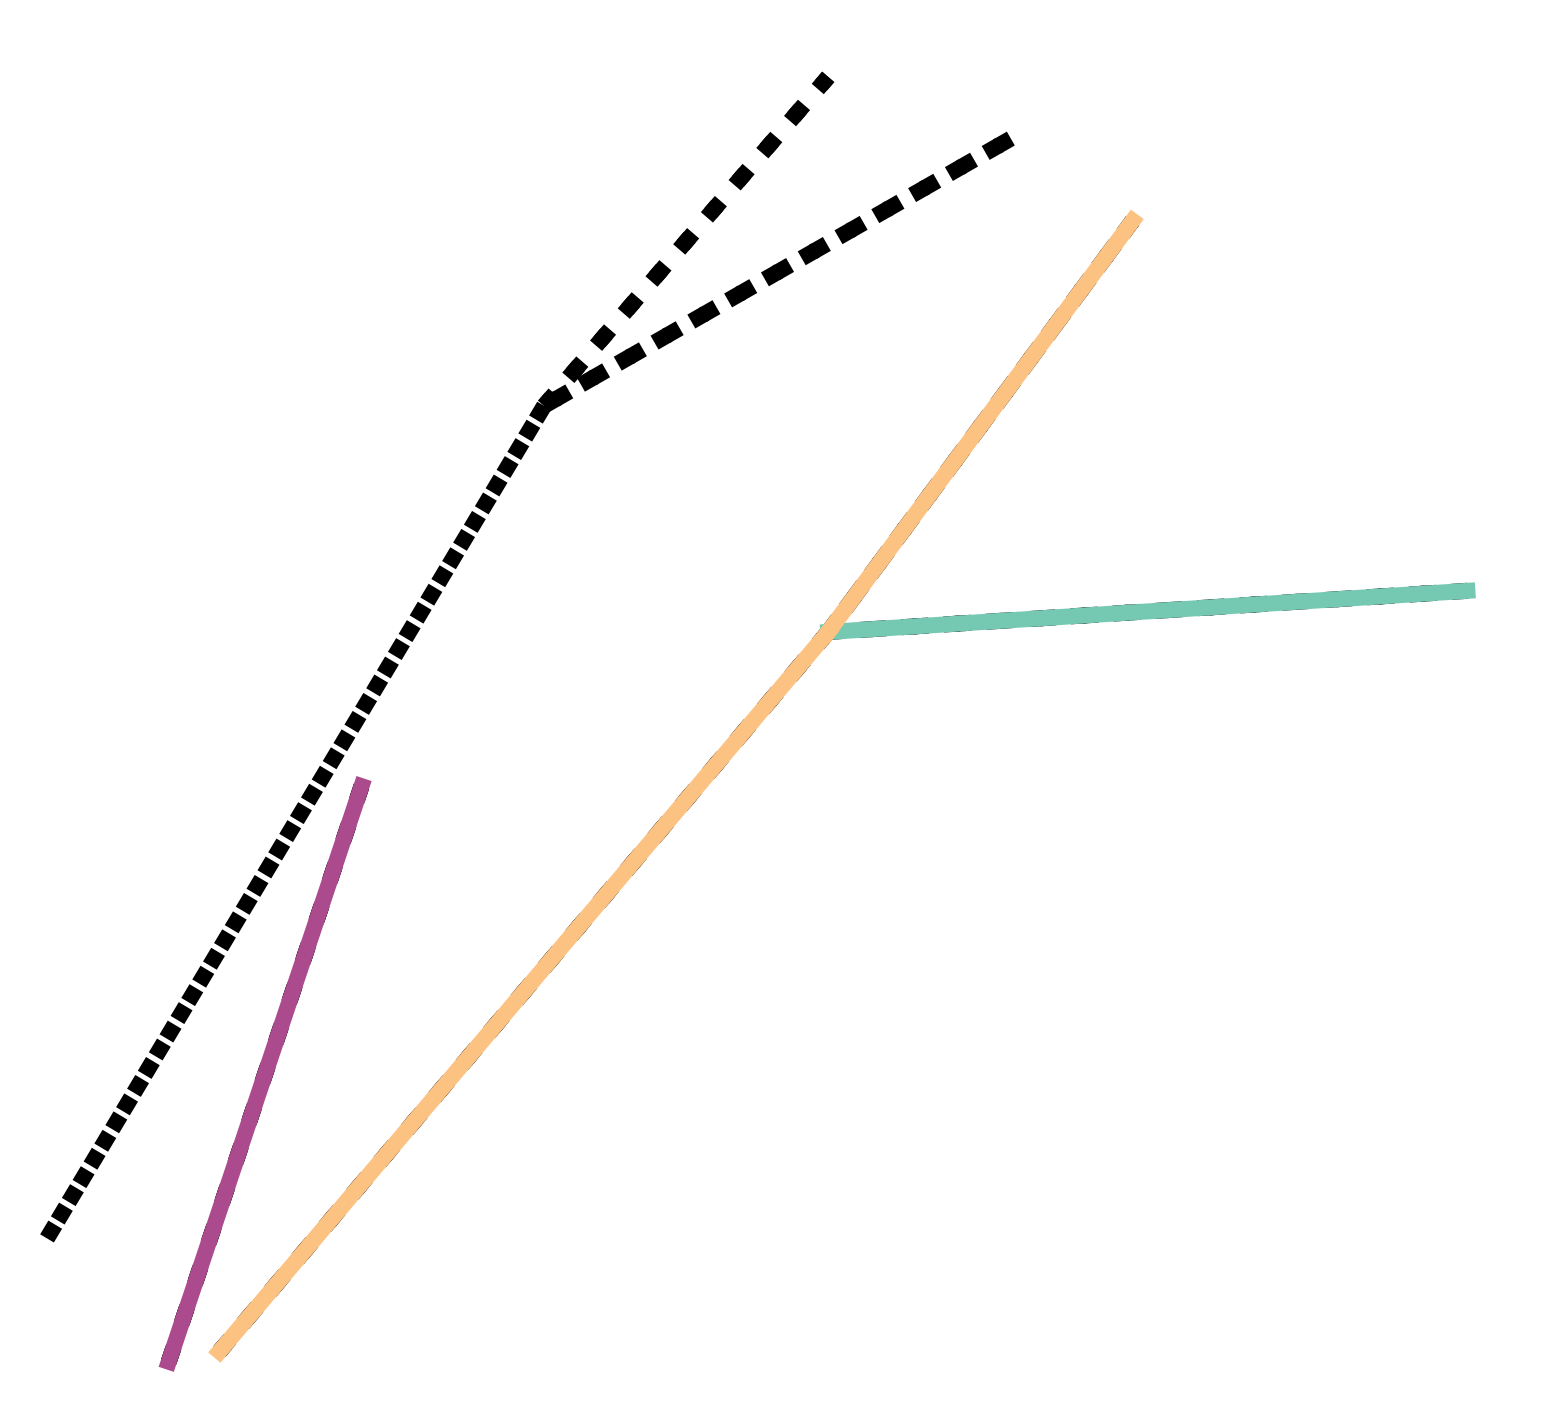
\includegraphics[height=1.5in]{resultImages/field3-t0-2cellBcrop-filtered-2-DeFiNeExactMatch-30.png}
        \caption{Filamentos correctamente individualizados por DeFiNe con 30\textdegree identificados con colores}
        \label{fig:field3t0filtered2Results-d}
    \end{subfigure}%
    ~ 
    \begin{subfigure}[t]{0.3\textwidth}
        \centering
        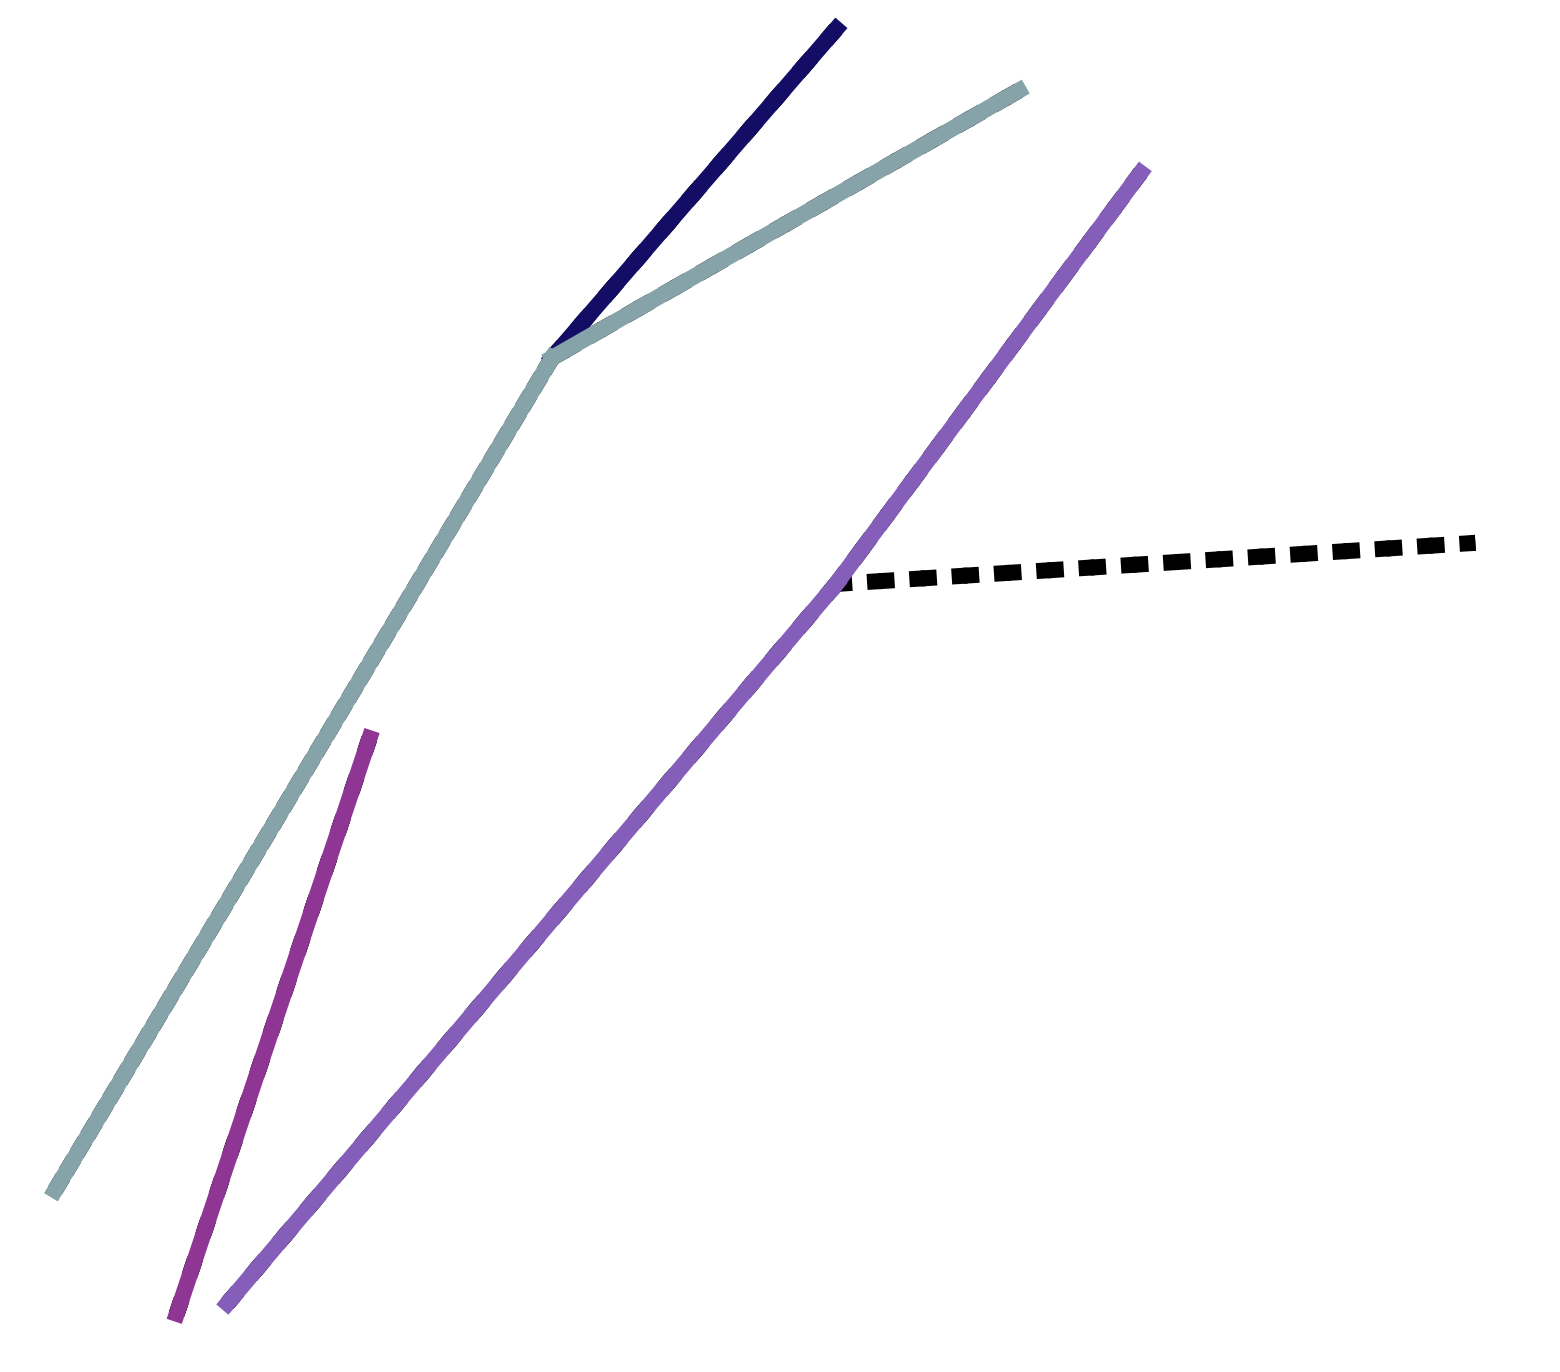
\includegraphics[height=1.5in]{resultImages/field3-t0-2cellBcrop-filtered-2-DeFiNeExactMatch-60.png}
        \caption{Filamentos correctamente individualizados por DeFiNe con 60\textdegree identificados con colores}
        \label{fig:field3t0filtered2Results-e}
    \end{subfigure}
    ~ 
    \begin{subfigure}[t]{0.3\textwidth}
        \centering
        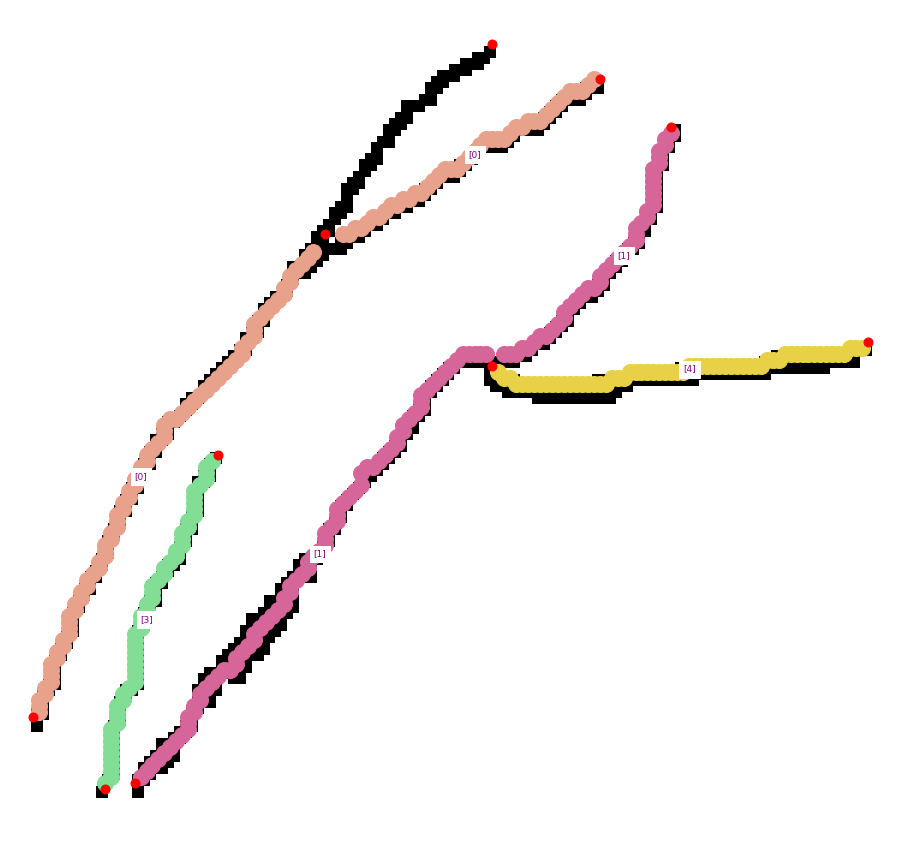
\includegraphics[height=1.5in]{resultImages/field3-t0-2cellBcrop-filtered-2-phil-s1271-v05-exactMatch-antLabeled.png}
        \caption{Filamentos correctamente individualizados por Phil identificados con colores}
        \label{fig:field3t0filtered2Results-f}
    \end{subfigure}
    
    \caption{Individualizaci\'on de filamentos realizadas con DeFiNe y Phil. Segmentos marcados en negro con y sin discontinuidad representan aristas no asignadas correctamente al filamento correspondiente en el {\it ground truth.}.}
    \label{fig:field3t0filtered2Results}
\end{figure*}

\begin{table}[h]
    \centering
    \begin{tabular}{|c|c|c|c|c|c|c|c|c|c|c|}
    \hline
        Algoritmo & VI & TP & FP &TN &FN & Rand	& Jaccard &	Precision &	Recall &	F1 \\ \hline
        Define 30° & 0.5714 & 1 & 1 & 18 & 1 & 0.9047 & 0.3333 & 0.5      & 0.5 & 0.5\\
        Define 60° & 0.4285 & 2 & 1 & 23 & 2 & 0.8928 & 0.4 & 0.6666 & 0.5 & 0.5714\\ 
        Phil & 0.4285  & 2 & 1 & 23 & 2 & 0.8928 & 0.4 & 0.6666 & 0.5 & 0.5714\\
        \hline
    \end{tabular}
    \caption{Resultados de individualizaci\'on de filamentos para figura \ref{fig:field3t0filtered2}. El valor m\'aximo de VI en este caso es de 1.9459, ya que el tama\~no del {\it data set} es de 7 aristas. El n\'umero de filamentos en el {\it ground truth} es 5.}
    %\label{tab:field3t0filtered2}
\end{table}
\addtocounter{table}{-1}
\begin{table}[h]
    \centering
    \begin{tabular}{|c|c|c|c|c|c|c|}
    \hline
         & \multirow{4}{2cm}{\centering \% Cobertura de Aristas} & \multirow{4}{2cm}{Filamentos Propuestos} & \multirow{4}{2cm}{Filamentos Correctos} & \multirow{4}{2.5cm}{\% Correctos vs Propuestos} & \multirow{4}{2.5cm}{\centering \% Correctos vs {\it Ground Truth}} & \multirow{4}{1.2cm}{\centering Tiempo [seg]} \\
         &  &  &  & & &  \\
        Algoritmo &  &  &  & & &  \\
        &  &  &  & & &  \\ \hline
        Define 30° & 1 & 5 & 3 & 60 & 60 & 2.8262\\
        Define 60° & 1 & 5 & 4 & 80 & 80 & 2.6506\\ 
        Phil & 1 & 5 & 4 & 80 & 80 & 0.2914\\
        \hline
    \end{tabular}
    \caption{Resultados ({\it Continuaci\'on}) de individualizaci\'on de filamentos para figura \ref{fig:field3t0filtered2}. El n\'umero de filamentos en el {\it ground truth} es 5.}
    %\label{tab:field3t0filtered2-2}
\end{table}

\subsection{Neuronas}